\begin{figure}[t]
\centering
\subfigure{\centering 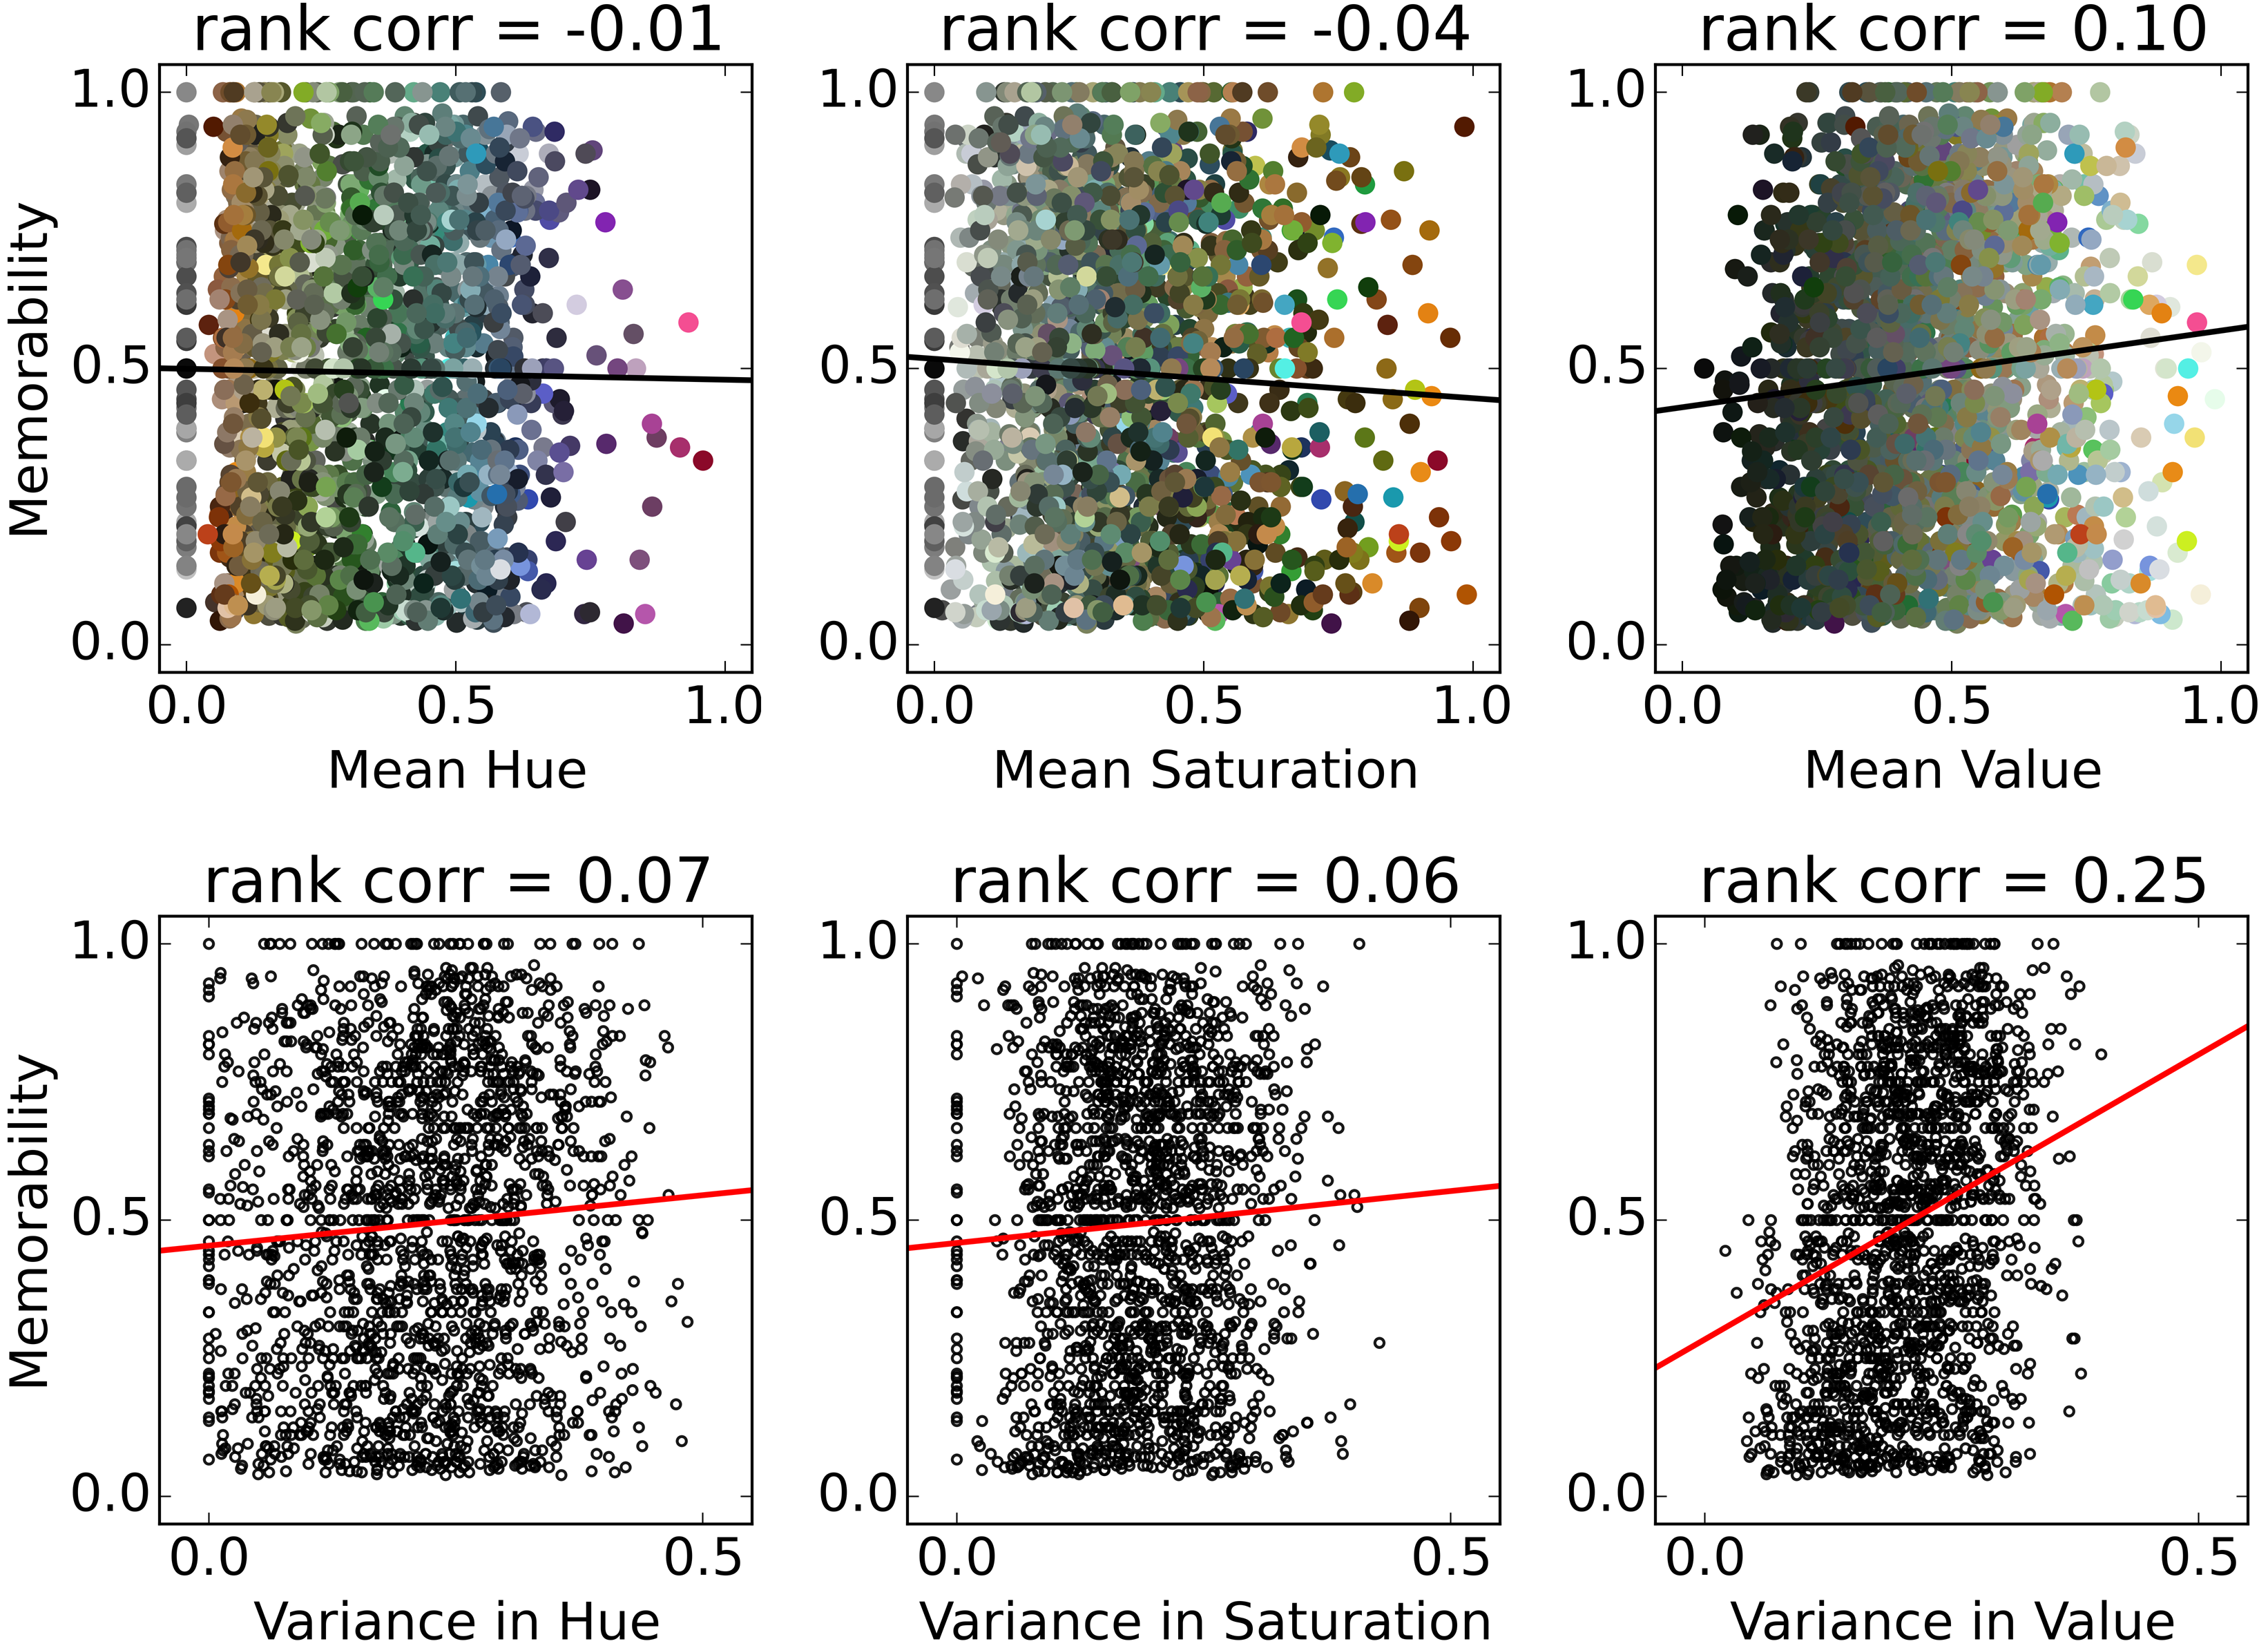
\includegraphics[width=0.45\textwidth]{figures/results/simple_features/color_corrs.png}}
\vspace{-5mm}\caption{\footnotesize\textbf{Correlations between simple color features and object memorability.} Color features were computed from HSV representations of the objects. }\label{fig:simple}
\end{figure}

While simple image features are traditionally poor predictors of memorability in full images \cite{isola11}, and with good reason \cite{konkle10}, do they play any role in determining object memorability? We decomposed each image into it's hue, saturation, and value components and calculated the mean and standard deviation of each channel. Mean value ($\rho = 0.1$) and variance in value ($\rho=0.25$) were weakly correlated with object memorability suggesting that brighter and higher contrast objects may be more memorable (Figure \ref{fig:simple}). On the other hand, essentially no relationship was found between memorability and either hue or saturation (Figure \ref{fig:simple}). This deviates slightly from the findings in \cite{isola11} that showed mean hue to be weakly predictive of image memorability. However, this makes sense since the effect was speculated to be due to the blue and green outdoor landscapes being less memorable than warmly colored human faces and indoor scenes. While our dataset contained plenty of indoor objects and people, outdoor scene-related image regions such as sky and ground were not included as objects. Taken together, these results show that, like image memorability, basic pixel statistics do not play a significant role in determining the memorability of objects in images.

